

%====================================================================================	 
\section{Related Work}

\subsection{Standards}
% \begin{frame}{Standards}
% 			\resizebox{10cm}{!} {
% 			\begin{tabular}{ll}
% 				\hline
% 				{\bf Code} & {\bf Title} \\ 
% 				\hline

% 				{\bf ICS 01. 110: Facilities Management} &  \\
% 				ISO/CD 18480-1  & Part 1: Terms and definitions \\
% 				ISO/CD 18480-2  & Part 2: Guidance on strategic sourcing and the development of agreements \\
% 				\hline

% 				% {\bf ICS 01. 110: Document Management} &  \\
% 				% EC 82045-1:2001  & Part 1: Principles and methods \\
% 				% IEC 82045-2:2004  & Part 2: Metadata elements and information reference model \\
% 				% ISO 82045-5:2005 & Part 5: Application of metadata for the construction and facility management sector \\ 
% 				% \hline

% 				{\bf ICS 03. 100: Risk Management} & \\
% 				ISO 31000:2009 & Principles and guidelines \\           
% 				ISO/TR 31004:2013  & Guidance for the implementation of ISO 31000 \\  		  
% 				IEC 31010:2009  & Risk assessment techniques \\  
% 				\hline

% 				% {\bf ICS 03. 100: Asset Management}  & \\
% 				% ISO 55000:2014 & Overview, principles and terminology \\ 	            
% 				% ISO 55001:2014 & Management systems-Requirements \\		            
% 				% ISO 55002:2014  & Management systems-Guidelines for the application of ISO 55001 \\  
% 				% \hline

% 				% {\bf ICS 03. 080: Outsourcing} & \\
% 				% ISO/DIS 37500 & Guidance on outsourcing \\ 
% 				% \hline

% 				% {\bf ICS 91. 010: Building Information Modeling} & \\
% 				% ISO/TS 12911:2012 & Framework for building information modeling (BIM) guidance \\ 		        
% 				% ISO 29481-1:2010 & Information delivery manual-Part 1: Methodology and format \\	            
% 				% ISO/AWI 29481-1 & Information delivery manual-Part 1: Methodology and format \\	            
% 				% ISO 29481-2:2012 & Information delivery manual-Part 2: Interaction framework \\
% 				% \hline

% 				% {\bf ICS 91. 040: Buildings and Building Related Facilities}  & \\  
% 				% ISO 11863:2011 & Functional and user requirements and performance -- Tools for assessment and comparison \\
% 				% \hline

% 				% {\bf ICS 91. 040: Buildings and Constructed Assets}  & \\
% 				% ISO 15686-1:2011 & Service life planning-Part 1: General principles and framework \\
% 				% ISO 15686-2:2012 & Service life planning-Part 2: Service life prediction procedures \\		            
% 				% ISO 15686-3:2002 & Service life planning-Part 3: Performance audits and reviews  \\		            
% 				% ISO/CD 15686-5 & Service life planning-Part 5: Life-cycle costing  \\         
% 				% ISO 15686-5:2008 & Service life planning-Part 5: Life-cycle costing  \\	            
% 				% ISO/AWI 15686--7 & Service life planning-Part 7: Performance evaluation for feedback of service life data from practice  \\		            
% 				% ISO 15686-7:2006 & Service life planning-Part 7: Performance evaluation for feedback of service life data from practice  \\	            
% 				% ISO 15686-8:2008 & Service life planning-Part 8: Reference service life and service--life estimation \\		            
% 				% ISO/TS 15686-9:2008 & Service life planning-Part 9: Guidance on assessment of service--life data  \\		            
% 				% ISO 15686-10:2010 & Service life planning-Part 10: When to assess functional performance \\		            
% 				% ISO/DTR 15686-11 & Service life planning-Part 11: Terminology \\
% 				% \hline

% 				% {\bf ICS 91. 040: Buildings Construction}  &  \\
% 				% ISO 15686-4:2014 & Service Life Planning -- Part 4: Service Life Planning using Building Information Modeling \\		            
% 				% ISO 6242-1:1992 & Expression of users' requirements-Part 1: Thermal requirements  \\		            
% 				% ISO 6242-2:1992 & Expression of users' requirements-Part 2: Air purity requirements  \\		            
% 				% ISO 6242-3:1992 & Expression of users' requirements-Part 3: Acoustical requirements \\
% 				% \hline

% 				{\bf ICS 91. 040: Performance Standards in Building}  & \\
% 				ISO 6240:1980 & Contents and presentation  \\	            
% 				ISO 6241:1984 & Principles for their preparation and factors to be considered  \\		            
% 				ISO 7162:1992 & Contents and format of standards for evaluation of performance  \\		            
% 				ISO 9699:1994 & Checklist for briefing-Contents of brief for building design  \\			            
% 				ISO 9836:2011 & Definition and calculation of area and space indicators \\
% 				\hline

% 			\end{tabular}
% 			}
% \end{frame}
% \note[itemize]{
% \item lista/tabela de standards e falo de 3 o 4 (ou parte da tabela) - ha standards disto, disto e disto, que familias de standards e que se aplicam, analisamos todos, e relativamente a este, existem estes todos. Nos standards de iso ha de facilities, maintenance, e cada um prescreve os indicadores X. Mostrar os indicadores que prescrevem.
% }

\begin{frame}{Standards}
	\fontsize{10}{8}\selectfont
	\vspace{-0.9cm}
	\begin{block}{ISO - International Organization for Standardization}
		\begin{itemize}
			\item ISO 31000:2009: Principles and guidelines           
		  	\item IEC 31010:2009: Risk assessment techniques
		\end{itemize}
	\end{block}
	\begin{block}{ICS - International Classification for Standards}
				\begin{itemize}
					\item ICS 03. 100: Risk Management
					\item ICS 01. 110: Facilities Management
				\end{itemize}
	\end{block}
	\begin{block}{RICS - Royal Institution of Chartered Surveyors}
				\begin{itemize}
					\item Gross External Areas (GEA)
					\item Net Internal Area (NIA)
				\end{itemize}
	\end{block}
	\begin{block}{BICS - Building Cost Information Service}			
			\begin{itemize}
					\item Occupancy costs
					\item Construction duration
			\end{itemize}
	\end{block}

\end{frame}
\note[itemize]{
	\item ISO: desenvolve standards internacionais para negocio e tecnologia - ISO de Risk Management
	\item ICS: Existem centenas de standards ISO, mas não se percebe quais se aplicam ao FM. É para isso que serve o ICS, para se ir busca-los mais facilmente. - cataloga os standards de acordo com as suas funções
	\item RICS:  É necessário existirem formas standard para critérios de medições, para que medições por exemplo de espaço, sejam feitas da mesma forma em todas as organizações. A RICS é uma instituição onde especialistas na área normalizam estas medições, e dão opniões imparciais relativamente a elas.
						\item Gross External Areas (GEA): Area medida or fora do edificio
						\item Net Internal Area (NIA): Area medida pelo lado de dentro do edificio, sem contar com a grossura das paredes externas
	\item BICS: standardiza os custos. Estabelece critérios para os custos. Pertencem ao RICS e providenciam concelhos de custos de ocupação, duração de construção de um edificio, etc Por exemplo, através de um custo standard por $m^2$, é possivel existirem edificios a um custo conhecido
}

\subsection{Scientific Literature}
\begin{frame}{Scientific Literature}
	\begin{itemize}
			\item Massheder and Finch, 1998
		\end{itemize}
		\begin{itemize}
			\item Ho et al, 2000
		\end{itemize}
		\begin{itemize}
			\item Costa et al, 2004
		\end{itemize}
		\begin{itemize}
			\item Hinks and McNay, 1999
		\end{itemize}
\end{frame}
\note[itemize]{
\item Há muito pouco trabalho cientifico relacionada a FM e benchmarking
\item
\item Conseguimos apenas encontrar 4 trabalhos relacionados com este tema: Massheder and Finch, Ho e outros, Costa e outros e Hinks and McNay.
\item
\item Todos eles tentam econtrar a lista de KPIs optima a ser utilizada pelas organizações.
}

\begin{frame}{Scientific Literature}
	\begin{block}{Massheder and Finch, 1998}
		\begin{itemize}
			\item Measure of the use of the different metrics on UK benchmarking organizations
		\end{itemize}
		\begin{itemize}
			\item The most used metrics are within the categories: Business, Portfolio Metrics and Building Performance
		\end{itemize}
	\end{block}
\end{frame}
\note[itemize]{

\item Massheder and Finch
\item Mediram a utilização de métricas em organizações de benchmarking no Reino Unido
\item Fizeram um questionário às 100 organizações de topo dos UK
\item As métricas mais utilizadas pertenciam às categorias de: Business, Portfolio Metrics and Building Performance

}

\begin{frame}{Scientific Literature}
	\vspace{-0.7cm}
	\begin{block}{Ho et al, 2000}
		\begin{itemize}
			\item Rates the importance of 97 metrics on a five point scale in Asia Pacific Region
		\end{itemize}

		\begin{figure}
		  \centering
		  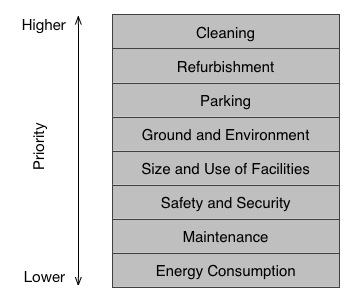
\includegraphics[width=0.4\textwidth]{images/MeasurementCatPriority.jpg}
		  \label{fig:MeasurementCatPriority}
		\end{figure}

		\begin{itemize}
			\item Most important metrics to the organizations: the ones with a financial implication
		\end{itemize}
	\end{block}
\end{frame}
\note[itemize]{
\item Fazem um raking das 97 métricas mais importantes na região da Ásia e Pacifico
\item Concluiram que as métricas mais importantes para as organizações estavam directamente implicadas com a parte financeira
}

\begin{frame}{Scientific Literature}


	\begin{block}{Costa et al, 2004}
		\begin{itemize}
			\item Discussion about three benchmarking initiatives in United Kingdom, United States of America and Chile
			%\item Each previous study selected the KPIs by combining distinct approaches: extensive reviews by a panel of experts and the publication of an initial report, selection based on previous studies, or by a committee involving both industry representatives and Construction Industry Institute
		\end{itemize}
		\begin{itemize}		
			\item Costa et al concluded that: 
			\begin{itemize}
				\item KPI selections were focused on categories such as Financial, Safety, Satisfaction and Performance
				\item The measures should be simple and well designed and give a comprehensive company wide-view 
			\end{itemize}
		\end{itemize}
	\end{block}
\end{frame}
\note[itemize]{
\item Discussão sobre 3 iniciativas de benchmarking: no Reino Unido (Key Performance Indicators Working Group, 2000), Estados Unidos (Construction Industry Institute, 2000) e Chile (Corporacion de Desarrolo Tecnológico, 2002)

\item Cada um dos estudos, seleccionou os KPIs de forma diferente: Reviews extensivas por experts;Selecção baseada em estudos anteriores, ou por um comité envolvendo representantes de várias industrias (Construction Industry Institute)
\item Costa et al concluiu: 
\begin{itemize}
	\item A selecção de KPIs focava-se nas categorias: Financeira (Desvio de custos por projecto), Segurança (Percentagem de Acidentes de Trabalho), Satisfação (deClientes e Empregados) and Performance (Project Schedule Growth)
	\item O conjunto de medições deve ser simples e bem desenhadas para suportar um melhoramento e dar uma VISAO ABRANGENTE compreensivel da empresa 
\end{itemize}
}

\begin{frame}{Scientific Literature}
	\begin{block}{Hinks and McNay, 1999}
		\begin{itemize}
			\item Need to established a set of universally accepted KPI
			\item {\bf First phase} literature review
			\item {\bf Second phase} questionnaires, scenario workshops and group discussions set
			\item {\bf Third phase} it was allocated a grade for each KPI, according to its importance
			\item Of 172 KPIs were selected the 23 most important
		\end{itemize}
	\end{block}
\end{frame}
\note[itemize]{
	\item Também Hinks and McNay identificaram uma necessidade de estabelecer um conjunto de KPIs universalmente aceitados
	\item
	\item {\bf First phase} Review de literatura cientifica
	\item
	\item {\bf Second phase} Foram feitos questionários, workshops e discussões em grupo a pessoas de dif. organizações
	\item
	\item {\bf Third phase} A cada KPI foi dada uma nota de acordo com as suas importancias
	\item
	\item Dos 172 KPIs seleccionaram-se os 23 mais importantes
}

\begin{frame}{Scientific Literature}
		\vspace{-0.5cm}
		\begin{figure}
		  \centering
		  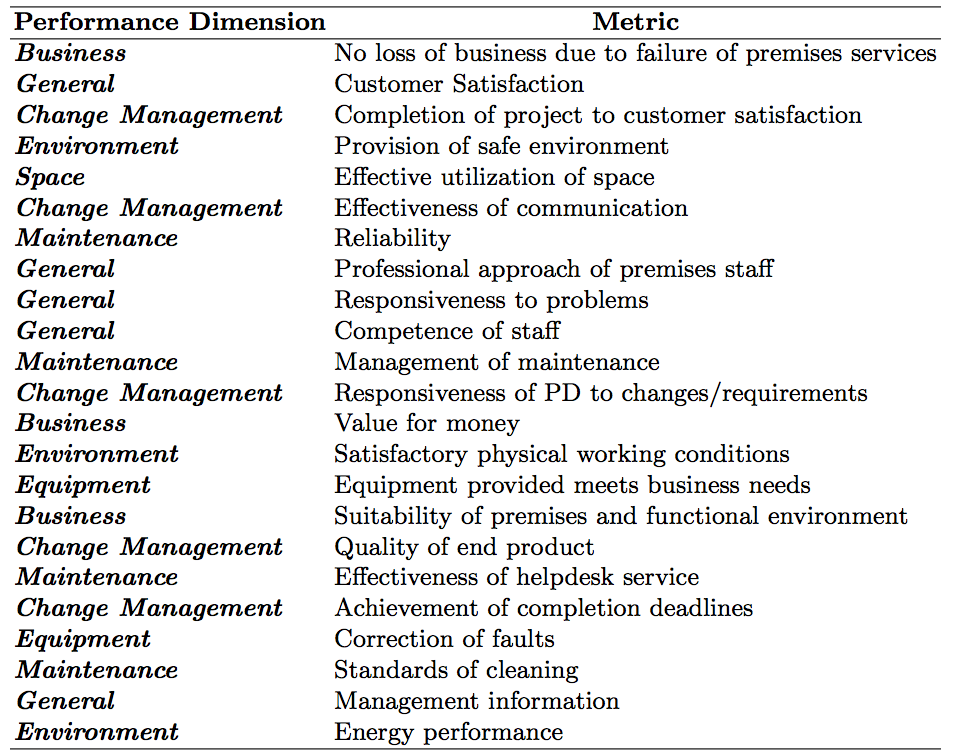
\includegraphics[width=0.9\textwidth]{images/23KPI.png}
		\end{figure}
\end{frame}
\note[itemize]{
\item Como podemos verificar, as métricas mais importantes centram-se na:
\item
\item Satisfação do cliente, 
\item
\item Segurança no trabalho e  
\item
\item Eficiência do business
\item
\item Rentabilização do espaço
}

\subsection{Existing Software Solutions}
\begin{frame}{Existing Software Solutions}
	% \begin{itemize}
	% 	\item Maxpanda or IBM Tririga make management more efficient: business analytics, critical alert, increasing visibility and control
	% \end{itemize}
	% \begin{itemize}
	% 	\item ARCHIBUS or FM:Systems have integration with CAD or BIM models
	% \end{itemize}
	% \begin{itemize}
	% 	\item FM solutions promote their capabilities for organizations cost reduction and user usability
	% \end{itemize}
	% \begin{itemize}
	% 	\item Systems like Indus Systems, Manhattan Mobile Apps, PNMSoft or ARCHIBUS have cloud-based software
	% \end{itemize}
	\resizebox{9cm}{!}{
	\begin{tabular}{p{6cm}llllllp{1cm}lr}
		\hline
		 {\bf Software Solutions} &  \begin{sideways}{\bf Centralization of Organizations Info}\end{sideways} 
		 & \begin{sideways}{\bf Business Analysis}\end{sideways} & \begin{sideways}{\bf Increased Visibility and Control}\end{sideways} & \begin{sideways}{\bf Costs Reduction}\end{sideways} & \begin{sideways}{\bf CAD/BIM Integration}\end{sideways} & \begin{sideways}{\bf Cloud Application}\end{sideways} & \begin{sideways}{\bf Benchmarking}\end{sideways} \\ 

		\hline
		Maxpanda 				& $\bullet$ & $\bullet$ & $\bullet$ & $\bullet$ & & & \\
		IBM Tririga 			& $\bullet$ & $\bullet$ & $\bullet$ & $\bullet$ & & & \\
		FM:Systems 				& $\bullet$ & $\bullet$ & $\bullet$ & $\bullet$ & $\bullet$ & & \\
		Indus System			& $\bullet$ & $\bullet$ & $\bullet$ & $\bullet$ & & $\bullet$ & \\
		PNMSoft 				& $\bullet$ & $\bullet$ & $\bullet$ & $\bullet$ & & $\bullet$ & $\bullet$ \\
		ARCHIBUS 				& $\bullet$ & $\bullet$ & $\bullet$  & $\bullet$ & $\bullet$ & $\bullet$ & $\bullet$ \\
		\hline
	\end{tabular}
	}
\end{frame}
\note[itemize]{
%\item Existem muitos softwares de soluções FM como CAFM ou BIM.

\item ---> Fazer TABELA
\item Soluções de FM como Maxpanda ou IBM Tririga tornam o FM mais fácil, já que centralizam a informação da organização, tornando a sua gestão mais eficiente através de analises do negócio, alertas e um aumento na visibilidade e controlo da organização.
\item Outras, como o ARCHIBUS ou o FM:Systems têm integração com modelos de CAD ou BIM. Isto torna possível a verificação da ocupação de departamentos, salas, ou outros espaços, o que é muito importante para a gestão de ocupação de areas.
\item Muitos destes sistemas promovem a redução de custos das organizações, já que conseguem justificar os custos de manutenção preventiva e conseguem prever um custo nas alterações da manutenção. 
\item Alguns focam-se em mais do que um sector e outros focam-se em mais do que um
\item Alguns sistemas como a Indus System, Manhattan Mobile Apps, PNMSoft ou ARCHIBUS tem um software baseado na cloud. Indus System enables users to store, share, view drawings, space, assets, related costs, leases and contracts just bye accessing the browser.
\item Por outro lado, ARCHIBUS e PNMSoft permitem mostrar os KPIs de organizações quando se acede aos seus sites. 
}

\begin{frame}
	\begin{block}{The Problem Remains}
	\begin{itemize}
		\item ARCHIBUS and PNMSoft show an organization KPIs when accessing their web site
	\end{itemize}
	\begin{itemize}
		\item Only applicable for facilities that have one of those software installed
	\end{itemize}
	\end{block}
\end{frame}
\note[itemize]{
\item Apesar do ARCHIBUS e o PNMSoft mostrarem os KPIs da organização, apenas funciona para comparações de uma facility ao longo do tempo, além disso, apenas funciona para quem tem esse software

%In contrast, with our solution, any organization could benefit from this features and one more: the comparison with others organizations on the sector.
}

\begin{frame}{Frequency of KPIs on Scientific Literature and Existing Solutions}
	\resizebox{8cm}{!}{
	\begin{tabular}{p{6cm}llllllp{1cm}lr}
		\hline
		 {\bf Indicators} &  \begin{sideways}{\bf Costa et al}\end{sideways} & \begin{sideways}{\bf USA, UK and Chile Projects}\end{sideways} & \begin{sideways}{\bf IFMA}\end{sideways} & \begin{sideways}{\bf ARCHIBUS}\end{sideways} & \begin{sideways}{\bf Ho et al}\end{sideways} & \begin{sideways}{\bf Massheder et al}\end{sideways} & \begin{sideways}{\bf Hinks et al}\end{sideways} & {\bf Total} \\ 

		\hline
		{\bf Financial Indicators} 	& & & & & & & & \\
		Total Cleaning Cost 				& & &$\bullet$ & & & & & 1 \\
		Cleaning Cost per $m^2$ 			& & &$\bullet$ &$\bullet$ & & & & 2 \\
		Total Maintenance Cost 				& & &$\bullet$ &$\bullet$ &$\bullet$ & & & 3 \\
		\hline
		{\bf Spacial Indicators}	& & & & & & & & \\
		Net Floor Area 						& & &$\bullet$ &$\bullet$ &$\bullet$ &$\bullet$ &$\bullet$ & 5  \\
		Percentage Net Floor Area 			& & &$\bullet$ &$\bullet$ &$\bullet$ & &$\bullet$ & 4 \\
		Percentage Internal Area			& & &$\bullet$ &$\bullet$ &$\bullet$ & &$\bullet$ & 4 \\
		\hline
		{\bf Maintenance/Cleaning Indicators}							& & & & & & & & \\
		Repairs VS Preventive Maintenance 										& & & & &$\bullet$ & &$\bullet$ & 2 \\
		Asset Replacement Values												& & &$\bullet$ & & & &$\bullet$ & 2 \\
		Percentage of Area Cleaned			 									& & &$\bullet$ & & & &$\bullet$ & 2 \\
		\hline
		 ... & & & ... & & & & & \\
	\end{tabular}

	}

\end{frame}
\note[itemize]{
\item E agora como podemos comparar estes trabalhos falados?
\item Aquilo que fizemos foi fazer uma apanhado de todos os KPIs referidos anteriormente e organizamo-los segundo a frequencia que surgiam nas diferentes fontes
\item Na vertical podemos ver as várias fontes
\item Na horizontal podemos ver os vários KPIs e as suas catgorias
\item Para chegar a esta matrix, foi necessário fazer uma normalização, pois existiam indicadores que surgiam com nomes diferentes em diferentes fontes
}

\begin{frame}{Calculation of KPIs}
	\resizebox{10cm}{!} {
	\begin{tabular}{llp{8cm}l}
		\hline
		 {\bf Indicators} &  {\bf Units} & {\bf Description} \\
		\hline
		{\bf Financial Indicators} & & \\
		Total Cleaning Cost 				& \euro/mo &  Sum of all cleaning costs \\
		Cleaning Cost per $m^2$ 			& \euro/$m^2$ &  Total Cleaning Cost/Net Room Area OR Total Cleaning Costs/Net Floor Area\\
		\hline
		{\bf Spacial Indicators} & & \\
		Net Floor Area per FTE				& $m^2$/FTE & Net Floor Area/Number of FTE personnel \\
		Percentage Net Floor Area 			& \% & (Net Floor Area/Total Level Area)x100 \\
		Percentage Internal Area			& \% & (Internal Area/Total Level Area)x100 \\
		\hline
		{\bf Maintenance/Cleaning Indicators} & & \\
		Repairs VS Preventive Maintenance (by specialty)						& \% & (Number of Corrective Maintenance per month/Number of Preventive Maintenance per month)x100 \\
		Asset Replacement Values (by specialty)												& \% & (Annual Maintenance Cost/Maintained Assets Replacement Value)x100\\
		Percentage of Area Cleaned 												& \% & Area Cleaned/Net Floor Area \\
		\hline
		... & ... & \\
	\end{tabular}
	}
\end{frame}
\note[itemize]{
\item Os indicadores especificados anteriormente, têm unidades especificas e medidas especificas utilizadas nos seus calculos
}

\begin{frame}{Discussion}
\vspace{-0.5cm}
\begin{figure}
  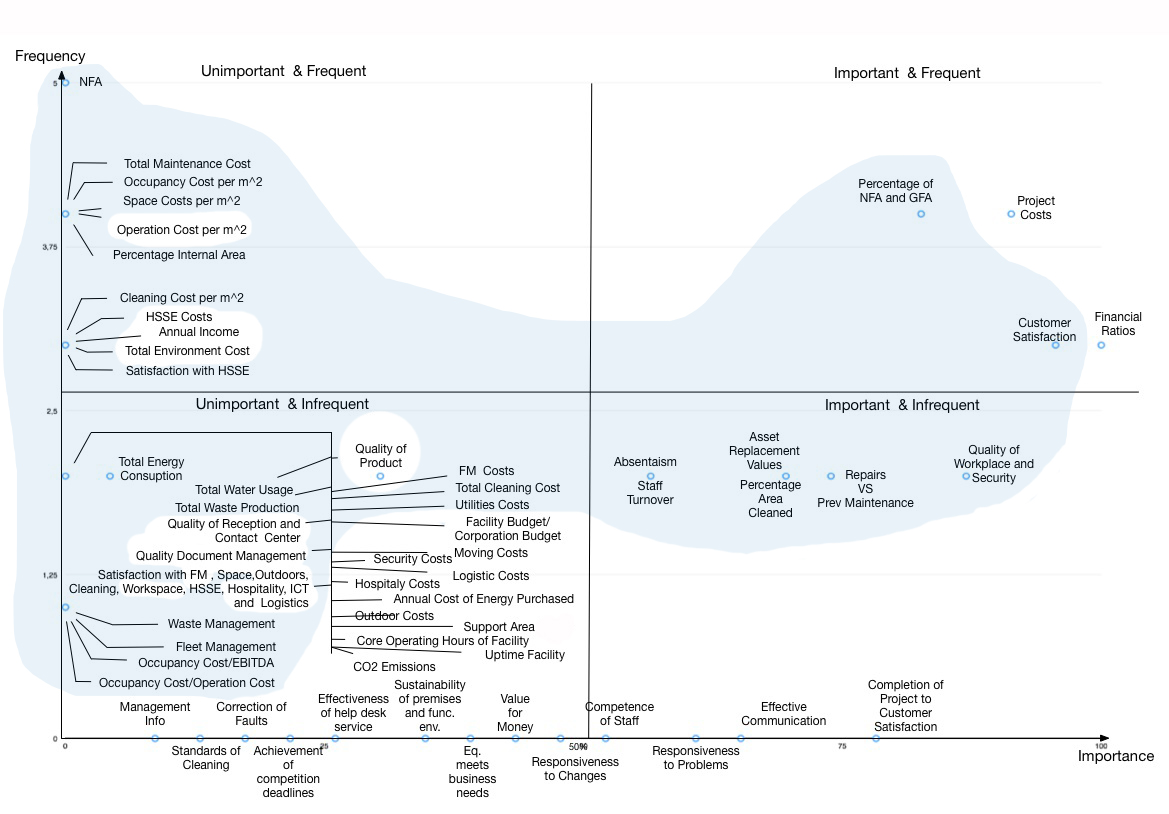
\includegraphics[width=1\textwidth]{images/importanceXfrequency10.jpg}
  \label{fig:importanceXfrequency}
\end{figure}

\end{frame}
\note[itemize]{
\item Fizemos o cruzamento dos dados da tabela de frequencia de kpis e a tabela da importancia dos kpis de hinks e mcnay
\item Se colocarmos todos os indicadores de acordo com a importancia e frequencia, obtemos este gráfico
\item Podemos distinguir 4 regiões, no canto direito superior temos os mais frequentes e mais importantes
\item No canto inferior esquerdo temos os menos importantes e menos frequentes
\item Faltaria validar esta distribuição atraves da opniaio de especialistas. Já fizesmos uma primeira abordagem a um especilista, onde concluimos que os indicadores mais indicados seriam os que estão dentro da mancha mais escura
}

\begin{frame}{KPIs Proposed}
	\vspace{-0.5cm}
	\resizebox{10cm}{!} {
	\begin{tabular}{llp{7cm}l}
		\hline
		 {\bf Indicator} &  {\bf Units} & {\bf Description} \\
		\hline
		{\bf Financial Indicators} & & \\
		Total Cleaning Cost 				& \euro/mo &  Sum of all cleaning costs \\
		Occupancy Cost per EBITDA & \% & (Occupancy Cost/Earning Before Interest, Taxes, Depreciation and Amortization)*100\\
		\hline

		{\bf Spacial Indicators} & & \\
		Net Floor Area per FTE				& $m^2$/FTE & Net Floor Area/Number of FTE personnel \\
		Percentage Gross Floor Area 		& \% & (Gross Floor Area/Total Level Area)x100 \\
		\hline
		{\bf Maintenance/Cleaning Indicators} & &  \\
		Repairs VS Preventive Maintenance (by specialty)						& \% & (Number of Corrective Maintenance per month/Number of Preventive Maintenance per month)x100 \\
		Percentage of Area Cleaned 												& \% & Area Cleaned/Net Floor Area \\
		\hline
		{\bf Productivity Indicators} & & \\
		Staff Turnover 	 			& \% & (Number of Employee Departures (FTE)/Average Number of Staff Members (FTE) Employed)x100\\
		Absenteeism  				& \% & (Total Days Lost/Total Possible Days Worked)x100 \\
		\hline

		{\bf Environmental Indicators} & & \\
		Total Energy Consumption	 		& kWh/mo & \\
		Total Water Usage					& $m^3$/mo & \\
		\hline
		 {\bf Service Quality Indicators} &  &  \\ 
		Quality of Cleaning							&  & Values Obtained Through Audits or Questionnaires \\
		Quality of Security 						&  & Values Obtained Through Audits or Questionnaires \\
		\hline
		... & ... & \\
	\end{tabular}
	}

\end{frame}
\note[itemize]{
\item Dessa lista dos kpis mais indicados para uma utilização acordada entre várias organizações, apresentamos aqui um exerto
}